\documentclass[12pt, titlepage]{article}

\usepackage{amsmath, mathtools}
\usepackage{amsfonts}
\usepackage{amssymb}
\usepackage[usenames,dvipsnames,table]{xcolor}
\usepackage{txfonts}
\usepackage[nocenter]{qtree}
\usepackage{xr}
\externaldocument{../SRS/SRS}
\newcommand{\rref}[1]{R\ref{#1}}
\newcommand{\ddref}[1]{DD\ref{#1}}

\usepackage{booktabs}
\usepackage{tabularx}
\usepackage{hyperref}
\hypersetup{
    colorlinks,
    citecolor=ForestGreen,
    filecolor=WildStrawberry,
    linkcolor=Purple,
    urlcolor=Cerulean
}
\usepackage[round]{natbib}
\usepackage{float}
\usepackage{listings}

%% Comments

\usepackage{color}

\newif\ifcomments\commentsfalse

\ifcomments
\newcommand{\authornote}[3]{\textcolor{#1}{[#3 ---#2]}}
\newcommand{\todo}[1]{\textcolor{red}{[TODO: #1]}}
\else
\newcommand{\authornote}[3]{}
\newcommand{\todo}[1]{}
\fi

\newcommand{\wss}[1]{\authornote{blue}{SS}{#1}}
\newcommand{\spc}[1]{\authornote{magenta}{SP}{#1}}

\newcommand{\progname}{Companion Cube Calculator} % PUT YOUR PROGRAM NAME HERE
\newcommand{\prognameAbbrv}{$C^{3}$}
\newcommand{\srsVersion}{2.0}

\begin{document}

\title{Test Plan for the \progname{} (\prognameAbbrv{}) Tool} 
\author{Geneva Smith}
\date{\today}
	
\maketitle

\pagenumbering{roman}

\section{Revision History}

\begin{tabularx}{\textwidth}{p{3.5cm}p{2cm}X}
\toprule {\bf Date} & {\bf Version} & {\bf Notes}\\
\midrule
December 19, 2017 & 2.0 & Updated plan to reflect current implementation \\
November 13, 2017 & 1.0.1 & Addition of missing test cases\\
October 25, 2017 & 1.0 & Initial draft completed\\
\bottomrule
\end{tabularx}

~\newpage

\section{Symbols, Abbreviations and Acronyms}

\renewcommand{\arraystretch}{1.2}
\begin{tabular}{l l} 
  \toprule		
  \textbf{Symbol} & \textbf{Description}\\
  \midrule 
  \prognameAbbrv{} & \progname{}\\
  GUI & Graphical User Interface\\
  IDE & Integrated Development Environment\\
  SRS & Software Requirements Specification\\
  T & Test\\
  \bottomrule
\end{tabular}\\

\newpage

\tableofcontents

\listoftables

\listoffigures

\newpage

\pagenumbering{arabic}

\section{General Information}
This document is a software test plan for the \progname{} (\prognameAbbrv{}), a 
mathematical tool which determines the range of a user-specified function given 
the domains of the function's variables. The calculations are performed using 
interval arithmetic.

\subsection{Purpose}
This document describes the software test plan for the \prognameAbbrv{} tool 
and is informed by its SRS documentation (version \srsVersion{}) and resulting 
implementation, including a description of automated testing approach, tools, 
and test cases. The purpose of documenting this information is to guide the 
product testing for the initial product release and to provide a basis for 
regression testing as further developments are made to the \prognameAbbrv{} 
tool.

This document is intended for readers who wish to test the initial version of 
the product, as well as those who want to refine and expand the tool. As 
changes are made to the \prognameAbbrv{} tool, these test cases will form the 
foundation of regression testing and will help ensure that any changes made to 
the product do not affect its original purpose or core functionality.

This test plan is intended to be used for version 1.0 of the \prognameAbbrv{} 
tool, and will only contain test information related to the product description 
in the product version's SRS documentation (version \srsVersion{}). Any 
functionality defined beyond the scope of the SRS document are not included in 
this version of the test plan.

All documentation and the associated release of the tool can be found at 
\href{https://github.com/GenevaS/CAS741}{https://github.com/GenevaS/CAS741}.

\subsection{Scope}
The \prognameAbbrv{} tool relies on interval arithmetic in the domain of real 
numbers ($\varmathbb{R}$), which means that many of its functions can be 
empirically tested. This plan contains testing for both specific and 
non-specific implementation aspects of the program. The implementation-specific 
tests are included to achieve 100\% code coverage to ensure that all code paths 
are reachable and produce expected outcomes. Non-specific implementation 
testing focuses on the correctness of the program with respect to its original 
purpose and its adherence to the SRS document.

The purpose of this plan is to modularize testing of the \prognameAbbrv{} 
tool so that it is easy to maintain and improve. It also forms the 
foundation of the kinds of behaviours that the tool should exhibit when it 
encounters malformed user inputs and unexpected values during its calculations.

\subsection{Overview of Document}
This document presents a general description of the \prognameAbbrv{} tool to 
establish the context of the test plan and a list of team members responsible 
for executing it. This background information is followed by a high-level 
description of the test plan, including the automated testing approach, 
verification tools, and non-testing based verification methods that will be 
used. The general plan outline is followed by a description of the system test 
which is designed to determine if the requirements from the associated SRS 
document are satisfied. The final section describes implementation-specific 
tests that were implemented to achieve 100\% code coverage.

\newpage

\section{Plan}
\label{testplan_highlevel}
This section describes the test plan for the \prognameAbbrv{} tool from a 
high-level perspective, outlining the methodologies and tools that will be used 
during the verification process, and the team responsible for executing the 
plan.
	
\subsection{Software Description}
The \prognameAbbrv{} tool is a stand-alone application for calculating
the mathematical range of a user-defined equation given the domains of
the equation's component variables. Equation ranges and variable
domains are represented by intervals, where intervals are defined as a
set of consecutive values bounded by a minimum and maximum value. The
minimum and maximum values for any given interval must be defined. To
perform its calculations, the \prognameAbbrv{} tool uses interval
arithmetic.

The purpose of this product is to produce accurate results when they can be 
found with respect to the host machine's floating-point precision. If a result 
cannot be found, the tool is expected to communicate the reason back to the 
user. Exact results are not required, as the tested equations are expected to 
the implemented in a software environment that has no impact on the external 
world. These tasks must be completed while presenting all communications to the 
user in standard function and interval notation.

\subsection{Test Team}

The test team assigned to implement this plan is Geneva Smith.

\subsection{Automated Testing Approach}
The \prognameAbbrv{} tool will almost exclusively rely on automated test 
approaches for its verification process, with the notable exceptions of the 
non-functional requirements for correctness, verifiability, usability and 
maintainability described in the SRS document (version \srsVersion{}). The 
verification of correctness cannot be tested by a machine because it relies on 
mathematical proofs and the remaining non-functional requirements of 
verifiability, usability, and maintainability are intended for a 
human audience. These types of verifications are best handled by manual tests 
and user studies.

The functional requirements tests (Section \ref{testplan_functional}) focus on 
the behaviour that is expected at each stage of the \prognameAbbrv{} tool's 
work flow. Since these behaviours are internal to the tool and do not require 
human guidance, these behaviours can be tested automatically using a series of 
black box unit tests. Some of the non-functional requirements such as 
robustness (Section \ref{testplan_nonfunctional}), can also be tested using 
automated approaches because they focus on empirically testable data, such as 
data constraints.

Many of the unit tests are designed to be used as part of integration testing, 
and the system will be progressively tested starting from the creation of data 
structures, to conversion processes, to input and output testing. Outputs 
include messages informing the user of erroneous behaviours or malformed 
inputs, and the calculated values and resulting equation tree if a no errors 
are detected.

The remaining unit tests are designed to test the correctness of the tool's 
calculation. Some of the tests check simple, two variable equations to ensure 
that the individual calculation types are behaving correctly. The remaining 
tests will ensure that equations with multiple operators are being decomposed 
correctly by comparing it to expected results. Once a set of equations has been 
selected for this task, regression testing becomes available to check further 
developments to the \prognameAbbrv{} tool.

\subsection{Verification Tools}
The C\# programming language has been chosen for the development of the 
\prognameAbbrv{} tool because of its GUI building capabilities. The supporting 
IDE, Visual Studio 2017 (Enterprise Edition), comes with a number of built-in 
test tools, including:

\begin{itemize}
	\item \textbf{A unit test framework and management system}\\
	This forms the bulk of the automated testing approach and will be used for 
	unit, integration, system, and regression testing. The IDE can be 
	configured so that existing unit tests are run automatically when the 
	program is compiled.
	\item \textbf{Code coverage tools}\\
	The code coverage tools in Visual Studio is connected to the test 
	management system and can help identify code that is not being run by any 
	unit test. 
\end{itemize}

\subsection{Non-Testing Based Verification}
There are a few non-functional requirements that cannot be tested 
automatically, but are still worth testing to verify their correctness:

\begin{itemize}
	\item Correctness can be tested using mathematical proofs to verify the 
	correctness of equation decomposition and order of operations.
	\item Verifiability, usability and maintainability can be verified using 
	user studies tailored for each requirement. This plan specifically contains 
	a user study description for the usability requirements 
	(Appendix~\ref{appendix_userstudy}).
\end{itemize}

\newpage

\section{System Test Description}
The system testing of the \prognameAbbrv{} tool will focus on inspecting and 
conditioning user inputs, verifying that the correct values are being produced 
by program calculations, and ensuring that the \prognameAbbrv{} tool is able to 
produce descriptive outputs for both valid and invalid inputs. These tests are 
divided into sections based on modules so that integration testing can arise 
naturally from the gradual addition of components. 

%The goal of user input inspection and conditioning tests is to be sure that 
%the 
%\prognameAbbrv{} tool is able to identify and reject values that violate the 
%assumptions. If the tool determines that the values do not violate the 
%assumptions, it should be able to convert those values into the internal 
%representations identified in the SRS document. For the purposes of this test 
%plan, it is assumed that the user function is represented internally as 
%a parse tree.
%
%Even if the user inputs are validated and conditioned correctly, it is still 
%possible for the \prognameAbbrv{} tool to encounter invalid operations in an 
%intermediary step while calculating a result. This makes it necessary to 
%create 
%a series of tests to determine how the tool will react to both supported and 
%unsupported operations.
%
%This test plan is meant to be executed in stages. The first stage is a 
%white-box unit test of the functionality required to get raw inputs from the 
%user. The subsequent stages are both integration and unit tests, where the 
%test 
%checks that the behaviour produced by the new modules is both working as 
%expected and can communicate with the modules above it. The final tests in 
%this 
%chain, which show the calculations of the \prognameAbbrv{} tool, form the 
%basis 
%of regression testing and contains mathematical functions that will be 
%incorrectly processed if the tool does not parse them correctly.
	
\subsection{Tests for Functional Requirements}
\label{testplan_functional}
The functional requirement tests are broken into four main groups. The 
``Getting User Inputs" tests (\ref{tests_gettingInputs}) test to make sure that 
no syntactic errors exist in the user's inputs that can be reasonably caught by 
the tool. The ``Conditioning User Inputs" tests convert the user's $D(v), v \in 
V$ into internal data structures and parses $f(V)$ into a semantically correct 
representation following BEDMAS rules. The ``Composing Operators" tests help 
prove that the composition of individual operators will produce the correct 
solution $R(f(V))$. Finally, the ``Presentation of Calculations to the User" 
tests ensure that the \prognameAbbrv{} tool follows the rules for significant 
figures and precision.

Each test case is associated with specific modules so that developers and 
maintainers have an idea of where to being their debugging process should a 
test fail.

\subsubsection{Getting User Inputs}
\label{tests_gettingInputs}
This test suite is designed to determine if the \rref{R_Inputs} (Accepting 
$f(V)$ and $D(v), v \in V$ as direct input or read from a file) functional 
requirement and any associated data constraints from \rref{R_verifyinputs} are 
satisfied.

Data that is read from a file is converted into the same format as the inputs 
for direct input methods, so they are not considered in the functional 
requirements testing explicitly. Complete unit tests for file I/O related 
functionality can be found in the User Input unit tests 
(Section~\ref{unit_inputs}).

\paragraph{User Input Tests}

\begin{enumerate}
	
	\item{test-directinput}
	
	Type: Functional, Automatic, System, Regression
		
	Initial State: New Session
		
	Input: \texttt{"x+y"}, \texttt{"x,2,4 \textbackslash ny,3,5"}
		
	Output: \texttt{"[5, 9]"}, \\
	\texttt{"+- \{+\}\\
		|     +- \{VAR\} x\\
		|     +- \{VAR\} y"}
		
	User Message: Range calculated successfully.
		
	How test will be performed: Unit Test
		
	Associated Module: Control Flow\\
	
	\item{test-input\_functionAsConstant}
	
	Type: Functional, Automatic, Integration
	
	Initial State: New Session
	
	Input: \texttt{"42"}
	
	Output:	$[42,42]$
	
	User Message: Warning: The user equation is a constant value and the range 
	will only include this value.
	
	How test will be performed: Unit Test
	
	Associated Module: Equation Conversion\\
\end{enumerate}

\paragraph{User Inputs (Missing, Incomplete, and Invalid Equation)}

\begin{enumerate}
	
	\item{test-input\_noFunction}
	
	Type: Functional, Automatic, Integration
	
	Initial State: New Session
	
	Input: \texttt{""}, \texttt{"x,2,4 \textbackslash ny,3,5"}
	
	Output: $successCode = -3$
	
	User Message: Error: Unrecognized sequence encountered during Atomic 
	Equation parsing. Remaining equation = 
	
	How test will be performed: Unit Test
	
	Associated Module: Control Flow\\
	
\end{enumerate}

\paragraph{User Inputs (Missing, Incomplete, and Invalid Domains)}

\begin{enumerate}
	
	\item{test-input\_noDomain}
		
	Type: Functional, Automatic, Integration
		
	Initial State: New Session
		
	Input: \texttt{"x+y"}, \texttt{"x,2,4"}
		
	Output:	$successCode = -2$
	
	User Message: Error: Cannot find intervals for variable name(s): y.
		
	How test will be performed: Unit Test
	
	Associated Module: Variable Consolidation\\
	
	\item{test-input\_nonNumberInDomain}
	
	Type: Functional, Automatic, Integration
	
	Initial State: New Session
	
	Input: \texttt{"x+y"}, \texttt{"x,2,4 \textbackslash ny,a,5"}
	
	Output: \Tree[.$+$ [.$x$  ] [.$y$  ] ], \{ \}
	
	User Message: Error: The string provided for the minimum bound cannot be 
	converted to a real number.
	
	How test will be performed: Unit Test
	
	Associated Module: Interval Conversion\\
	
	\item{test-input\_missingMinDomainValue}
	
	Type: Functional, Automatic, Integration
	
	Initial State: New Session
	
	Input: \texttt{"x+y"}, \texttt{"x,,4 \textbackslash ny,a,5"}
	
	Output: \Tree[.$+$ [.$x$  ] [.$y$  ] ], \{ x = [4,4], y = [3,5]\}
	
	User Message: Warning: No minimum interval bound given. Setting it to the 
	same value as the maximum bound.
	
	How test will be performed: Unit Test
	
	Associated Module: Interval Conversion\\
	
	\item{test-input\_missingMaxDomainValue}
	
	Type: Functional, Automatic, Integration
	
	Initial State: New Session
	
	Input: \texttt{"x+y"}, \texttt{"x,2,4 \textbackslash ny,3,"}
	
	Output: \Tree[.$+$ [.$x$  ] [.$y$  ] ], \{ x = [2,4], y = [3,3]\}
	
	User Message: Warning: No maximum interval bound given. Setting it to the 
	same value as the minimum bound.
	
	How test will be performed: Unit Test
	
	Associated Module: Interval Conversion\\
	
\end{enumerate}

\paragraph{User Inputs (Extraneous Information)}

\begin{enumerate}
	\item{test-input\_variableNotInFunction}
	
	Type: Functional, Automatic, Integration
	
	Initial State: New Session
	
	Input: \texttt{"x+y"}, \texttt{"x,2,4 \textbackslash ny,3,5 \textbackslash 
	nz,6,7"}
	
	Output: \Tree[.$+$ [.$x$  ] [.$y$  ] ], \{ x = [2,3], y = [4,5] \}
	
	User Message: Warning: Extraneous variables found in interval list (z).
	
	How test will be performed: Unit Test
	
	Associated Module: Variable Consolidation\\
	
\end{enumerate}

\paragraph{Variable Names}

\begin{enumerate}
	
	\item{test-input\_simpleVariableName}
	
	Type: Functional, Automatic, Integration
	
	Initial State: New Session
	
	Input: \texttt{"x+y"}
	
	Output: \texttt{\{ "x", "y" \}}
	
	User Message: - 
	
	How test will be performed: Unit Test
	
	Associated Module: Equation Conversion\\
	
	\item{test-input\_multiCharacterVariableName1}
	
	Type: Functional, Automatic, Integration
	
	Initial State: New Session
	
	Input: \texttt{"x1+y"}
	
	Output: \texttt{\{ "x1", "y" \}}
	
	User Message: - 
	
	How test will be performed: Unit Test
	
	Associated Module: Equation Conversion\\
	
	\item{test-input\_multiCharacterVariableName2}
	
	Type: Functional, Automatic, Integration
	
	Initial State: New Session
	
	Input: \texttt{"x\_+y"}
	
	Output: \texttt{\{ "x\_", "y" \}}
	
	User Message: - 
	
	How test will be performed: Unit Test
	
	Associated Module: Equation Conversion\\
	
	\item{test-input\_multiCharacterVariableName3}
	
	Type: Functional, Automatic, Integration
	
	Initial State: New Session
	
	Input: \texttt{"x\_1+y"}
	
	Output: \texttt{\{ "x\_1", "y" \}}
	
	User Message: - 
	
	How test will be performed: Unit Test
	
	Associated Module: Equation Conversion\\
	
	\item{test-input\_multiCharacterVariableName4}
	
	Type: Functional, Automatic, Integration
	
	Initial State: New Session
	
	Input: \texttt{"x\_i+y"}
	
	Output: \texttt{\{ "x\_i", "y" \}}
	
	User Message: - 
	
	How test will be performed: Unit Test
	
	Associated Module: Equation Conversion\\
	
	\item{test-input\_multiCharacterVariableName5}
	
	Type: Functional, Automatic, Integration
	
	Initial State: New Session
	
	Input: \texttt{"x``+y"}
	
	Output: \texttt{\{ "x``", "y" \}}
	
	User Message: - 
	
	How test will be performed: Unit Test
	
	Associated Module: Equation Conversion\\
	
	\item{test-input\_multiCharacterVariableName6}
	
	Type: Functional, Automatic, Integration
	
	Initial State: New Session
	
	Input: \texttt{"xy+y"}
	
	Output: \texttt{\{ "xy", "y" \}}
	
	User Message: - 
	
	How test will be performed: Unit Test
	
	Associated Module: Equation Conversion\\
	
%	\item{test-input\_multiCharacterVariableName7}
%	
%	Type: Functional, Automatic, Integration
%	
%	Initial State: New Session
%	
%	Input: $f(V) = xy$, $x = [2,4], y = [3,5]$
%	
%	Output: Warning -- Found variable $xy$ that does not exist in the domain 
%	list for $f(V)$ -\textgreater expanding to multiplication $x * y$
%	
%	How test will be performed: Unit Test
%	
%	Associated Module: \\
	
\end{enumerate}

\subsubsection{Conditioning User Inputs}
\label{tests_conditioningInputs}
This test suite is designed to determine if the \rref{R_conditionX} (Converting 
each $D(v)$ into \ddref{DD_interval}) and \rref{R_conditionfx} (Decomposing 
$f(V)$ into two-operand equations following BEDMAS rules) functional 
requirements and the associated data constraints from \rref{R_verifyinputs} are 
satisfied.

\paragraph{Unexpected Domain Ordering}

\begin{enumerate}
	
	\item{test-parse\_domainOrder}
	
	Type: Functional, Automatic, Integration
	
	Initial State: New Session
	
	Input: \texttt{"x,2,4 \textbackslash ny,3,-5"}
	
	Output:	$\{ x = [2,4], y = [-5,3] \}$
	
	User Message: WARNING: Value provided for intervals are not in increasing 
	order.The values have been exchanged to maintain the interval ordering.
	
	How test will be performed: Unit Testing
	
	Associated Module: Interval Data Structure\\
	
	\item{unittest-intervaldatastructuresethighmin}
	
	Type: Functional, Automatic, Unit
	
	Initial State: New Session
	
	Input: $x = [3,4]$
	
	Changes: $min = 5$
	
	Output: $x = [4,5]$
	
	User Message: WARNING: Value provided for minimum bound is greater than the 
	current maximum bound. The values have been exchanged to maintain the 
	interval ordering.
	
	How test will be performed: Unit Testing
	
	Associated Module: IntervalStruct\\
	
	\item{unittest-intervaldatastructuresetlowmax}
	
	Type: Functional, Automatic, Unit
	
	Initial State: New Session
	
	Input: $x = [3,4]$
	
	Changes: $max = -1$
	
	Output: $x = [-1,3]$
	
	User Message: WARNING: Value provided for maximum bound is smaller than the 
	current minimum bound. The values have been exchanged to maintain the 
	interval ordering.
	
	How test will be performed: Unit Testing
	
	Associated Module: IntervalStruct\\
	
\end{enumerate}

\paragraph{Creating Equation Trees}

\begin{enumerate}
	
	\item{test-parse\_addition}
	
	Type: Functional, Automatic, Integration
	
	Initial State: New Session
	
	Input: \texttt{"x+y"}
	
	Output: \Tree[.$+:$ [.$VAR:x$  ] [.$VAR:y$  ] ], \texttt{\{ "x", "y" \}}
	
	User Message: - 
	
	How test will be performed: Unit Testing
	
	Associated Module: Equation Conversion\\
	
	\item{test-parse\_subtraction}
	
	Type: Functional, Automatic, Integration
	
	Initial State: New Session
	
	Input: \texttt{"x-y"}
	
	Output: \Tree[.$-:$ [.$VAR:x$  ] [.$VAR:y$  ] ], \texttt{\{ "x", "y" \}}
	
	User Message: - 
	
	How test will be performed: Unit Testing
	
	Associated Module: Equation Conversion\\
	
	\item{test-parse\_multiplication}
	
	Type: Functional, Automatic, Integration
	
	Initial State: New Session
	
	Input: \texttt{"x*y"}
	
	Output: \Tree[.$*:$ [.$VAR:x$  ] [.$VAR:y$  ] ], \texttt{\{ "x", "y" \}}
	
	User Message: - 
	
	How test will be performed: Unit Testing
	
	Associated Module: Equation Conversion\\

	\item{test-parse\_division}
	
	Type: Functional, Automatic, Integration
	
	Initial State: New Session
	
	Input: \texttt{"x/y"}
	
	Output: \Tree[.$/:$ [.$VAR:x$  ] [.$VAR:y$  ] ], \texttt{\{ "x", "y" \}}
	
	User Message: - 
	
	How test will be performed: Unit Testing
	
	Associated Module: Equation Conversion\\
	
	\item{test-parse\_intervalexponents}
	
	Type: Functional, Automatic, Integration
	
	Initial State: New Session
	
	Input: \texttt{"2\textasciicircum x"}
	
	Output: \Tree[.$\wedge:$ [.$CONST:2$  ] [.$VAR:x$  ]  ], \texttt{\{ "x" \}}
	
	User Message: - 
	
	How test will be performed: Unit Testing
	
	Associated Module: Equation Conversion\\
	
	\item{test-parse\_intervalbase}
	
	Type: Functional, Automatic, Integration
	
	Initial State: New Session
	
	Input: \texttt{"x\textasciicircum 2"}
	
	Output: \Tree[.$\wedge:$ [.$VAR:x$  ] [.$CONST:2$  ]  ], \texttt{\{ "x" \}}
	
	User Message: - 
	
	How test will be performed: Unit Testing
	
	Associated Module: Equation Conversion\\
	
\end{enumerate}

\paragraph{Constant Values}

\begin{enumerate}
	
	\item{test-parse\_constantValue1}
	
	Type: Functional, Automatic, Integration
	
	Initial State: New Session
	
	Input: \texttt{"4+x"}
	
	Output: \Tree[.$+:$ [.$CONST:4$  ] [.$VAR:x$  ]  ], \texttt{\{ "x" \}}
	
	User Message: - 
	
	How test will be performed: Unit Testing
	
	Associated Module: Equation Conversion\\
	
	\item{test-parse\_constantValue2}
	
	Type: Functional, Automatic, Integration
	
	Initial State: New Session
	
	Input: \texttt{"-4+x"}
	
	Output: \Tree[.$+:$ [.$CONST:-4$  ] [.$VAR:x$  ] ], \texttt{\{ "x" \}}
	
	User Message: - 
	
	How test will be performed: Unit Testing
	
	Associated Module: Equation Conversion\\
	
	\item{test-parse\_constantValue3}
	
	Type: Functional, Automatic, Integration
	
	Initial State: New Session
	
	Input: \texttt{"x/-4"}
	
	Output: \Tree[.$/:$ [.$VAR:x$  ] [.$CONST:-4$  ] ], \texttt{\{ "x" \}}
	
	User Message: - 
	
	How test will be performed: Unit Testing
	
	Associated Module: Equation Conversion\\

	\item{test-parse\_constantValue4}
	
	Type: Functional, Automatic, Integration
	
	Initial State: New Session
	
	Input: \texttt{"x+4"}
	
	Output: \Tree[.$+:$ [.$VAR:x$  ] [.$CONST:4$  ] ], \texttt{\{ "x" \}}
	
	User Message: - 
	
	How test will be performed: Unit Testing
	
	Associated Module: Equation Conversion\\
	
	\item{test-parse\_constantValue5}
	
	Type: Functional, Automatic, Integration
	
	Initial State: New Session
	
	Input: \texttt{"x+-4"}
	
	Output: \Tree[.$+:$ [.$VAR:x$  ] [.$CONST:-4$  ] ], \texttt{\{ "x" \}}
	
	User Message: - 
	
	How test will be performed: Unit Testing
	
	Associated Module: Equation Conversion\\
	
	\item{test-parse\_constantValue6}
	
	Type: Functional, Automatic, Integration
	
	Initial State: New Session
	
	Input: \texttt{"x+42"}
	
	Output: \Tree[.$+:$ [.$VAR:x$  ] [.$CONST:42$  ] ], \texttt{\{ "x" \}}
	
	User Message: - 
	
	How test will be performed: Unit Testing
	
	Associated Module: Equation Conversion\\
	
	\item{test-parse\_implicitMultiplication}
	
	Type: Functional, Automatic, Integration
	
	Initial State: New Session
	
	Input: \texttt{"4x"}
	
	Output: \Tree[.$*:$ [.$CONST:4$  ] [.$VAR:x$  ] ], \texttt{\{ "x" \}}
	
	User Message: Warning: Encountered an implicit multiplication of a constant 
	value and a variable. Expanding with explicit operator.
	
	How test will be performed: Unit Testing
	
	Associated Module: Equation Conversion\\
	
\end{enumerate}

\paragraph{Precedence of Brackets}

\begin{enumerate}
	
	\item{test-parse\_brackets1}
	
	Type: Functional, Automatic, Integration
	
	Initial State: New Session
	
	Input: \texttt{"x+(y-z)"}
	
	Output: \Tree[.$+:$ [.$VAR:x$  ] [.$():$ [.$-:$ [.$VAR:y$ ] [.$VAR:z$ ] ] ] 
	]
	
	User Message: - 
	
	How test will be performed: Unit Testing
	
	Associated Module: Equation Conversion\\
	
	\item{test-parse\_brackets2}
	
	Type: Functional, Automatic, Integration
	
	Initial State: New Session
	
	Input: \texttt{"(x*y)-2\textasciicircum z"}
	
	Output: \Tree[.$-:$ [.$():$ [.$*:$ [.$VAR:x$  ] [.$VAR:y$  ]   ]  
	] [.$\wedge$ [.$CONST:2$ ] [.$VAR:z$  ]  ]	]

	User Message: - 
	
	How test will be performed: Unit Testing
	
	Associated Module: Equation Conversion\\
	
	\item{test-parse\_brackets3}
	
	Type: Functional, Automatic, Integration
	
	Initial State: New Session
	
	Input: \texttt{"w*(x/(y+z))"}
	
	Output: \Tree[.$*:$ [.$VAR:w$  ] [.$():$ [.$/:$ [.$VAR:x$ ] [.$():$ [.$+:$ 
	[.$VAR:y$  ] [.$VAR:z$  ] ]]   ]  ] 	]
	
	User Message: - 
	
	How test will be performed: Unit Testing
	
	Associated Module: Equation Conversion\\
	
\end{enumerate}

\paragraph{Open Brackets}

\begin{enumerate}
	
	\item{test-parse\_openLeftBracket}
	
	Type: Functional, Automatic, Integration
	
	Initial State: New Session
	
	Input: \texttt{"x+y-z)"}
	
	Output: $NULL$
	
	User Message: Error: Unrecognized sequence encountered during Atomic 
	Equation parsing. Remaining equation = )
	
	How test will be performed: Unit Testing
	
	Associated Module: Equation Conversion\\
	
	\item{test-parse\_openRightBracket}
	
	Type: Functional, Automatic, Integration
	
	Initial State: New Session
	
	Input: \texttt{"x+(y-z"}
	
	Output: $NULL$
	
	User Message: Error: Could not find the end of the equation.
	
	How test will be performed: Unit Testing
	
	Associated Module: Equation Conversion\\
	
\end{enumerate}

\subsubsection{Correctness of Component Calculations}
\label{tests_correctnessOfCalculations}
This test suite is designed to determine if the \rref{R_Calculate} 
(Solving each component equation in $f(V)$) and \rref{R_VerifyOutput} (Ensuring 
that the calculated result is represented in closed, interval form) functional 
requirements, and the associated data constraints from 
\rref{R_VerifyOutputConstraints} are satisfied.

\paragraph{Correctness of Addition, Subtraction, and Multiplication}

\begin{enumerate}
	
	\item{test-calculate\_addition}
	
	Type: Functional, Automatic, Integration
	
	Initial State: New Session
	
	Input: \Tree[.$+:$ [.$VAR:x$  ] [.$VAR:y$  ] ], $\{ x = [2,4], y = [3,5] \}$
	
	Output: $[5,9]$
	
	User Message: - 
	
	How test will be performed: Unit Testing
	
	Associated Module: Range Solver \\
	
	\item{test-calculate\_additionconstant}
	
	Type: Functional, Automatic, Integration
	
	Initial State: New Session
	
	Input: \Tree[.$+:$ [.$VAR:x$  ] [.$CONST:4$  ] ], $\{ x = [2,4] \}$
	
	Output: $[6,8]$
	
	User Message: - 
	
	How test will be performed: Unit Testing
	
	Associated Module: Range Solver\\
	
	\item{test-calculate\_subtraction}
	
	Type: Functional, Automatic, Integration
	
	Initial State: New Session
	
	Input: \Tree[.$-:$ [.$VAR:x$  ] [.$VAR:y$  ] ], $\{ x = [2,4], y = [3,5] \}$
	
	Output: $[-1,-1]$
	
	User Message: - 
	
	How test will be performed: Unit Testing
	
	Associated Module: Range Solver\\
	
	\item{test-calculate\_multiplication1}
	
	Type: Functional, Automatic, Integration
	
	Initial State: New Session
	
	Input: \Tree[.$*:$ [.$VAR:x$  ] [.$VAR:y$  ] ], $\{ x = [2,4], y = [3,5] \}$
	
	Output: $[6,20]$
	
	User Message: - 
	
	How test will be performed: Unit Testing
	
	Associated Module: Range Solver\\
	
	\item{test-calculate\_multiplication2}
	
	Type: Functional, Automatic, Integration
	
	Initial State: New Session
	
	Input: \Tree[.$*:$ [.$VAR:x$  ] [.$VAR:y$  ] ], $\{ x = [-1,3], y = [-3,5] 
	\}$
	
	Output: $[-9,15]$
	
	User Message: - 
	
	How test will be performed: Unit Testing
	
	Associated Module: Range Solver\\
	
	\item{test-calculate\_multiplication3}
	
	Type: Functional, Automatic, Integration
	
	Initial State: New Session
	
	Input: \Tree[.$*:$ [.$VAR:x$  ] [.$VAR:y$  ] ], $\{ x = [-3,-1], y = 
	[-5,-2] \}$
	
	Output: $[2,15]$
	
	User Message: - 
	
	How test will be performed: Unit Testing
	
	Associated Module: Range Solver\\
	
\end{enumerate}

\paragraph{Correctness of Division}

\begin{enumerate}
	
	\item{test-calculate\_divisionPositiveDivisor1}
	
	Type: Functional, Automatic, Integration
	
	Initial State: New Session
	
	Input: \Tree[.$/:$ [.$VAR:x$  ] [.$VAR:y$  ] ], $\{ x = [2,4], y = [3,5] \}$
	
	Output: $[0.4,1.3333333333333333]$
	
	User Message: - 
	
	How test will be performed: Unit Testing
	
	Associated Module: Range Solver\\
	
	\item{test-calculate\_divisionPositiveDivisor2}
	
	Type: Functional, Automatic, Integration
	
	Initial State: New Session
	
	Input: \Tree[.$/:$ [.$VAR:x$  ] [.$VAR:y$  ] ], $\{ x = [0,4], y = [3,5] \}$
	
	Output: $[0, 1.3333333333333333]$
	
	User Message: - 
	
	How test will be performed: Unit Testing
	
	Associated Module: Range Solver\\
	
	\item{test-calculate\_divisionPositiveDivisor3}
	
	Type: Functional, Automatic, Integration
	
	Initial State: New Session
	
	Input: \Tree[.$/:$ [.$VAR:x$  ] [.$VAR:y$  ] ], $\{ x = [-1,4], y = [3,5] 
	\}$
	
	Output: $[-0.3333333333333333,0.8]$
	
	User Message: - 
	
	How test will be performed: Unit Testing
	
	Associated Module: Range Solver\\

	\item{test-calculate\_divisionPositiveDivisor4}
	
	Type: Functional, Automatic, Integration
	
	Initial State: New Session
	
	Input: \Tree[.$/:$ [.$VAR:x$  ] [.$VAR:y$  ] ], $\{ x = [-2,0], y = [3,5]
	\}$
	
	Output: $[-0.6666666666666666,0]$
	
	User Message: - 
	
	How test will be performed: Unit Testing
	
	Associated Module: Range Solver\\
	
	\item{test-calculate\_divisionPositiveDivisor5}
	
	Type: Functional, Automatic, Integration
	
	Initial State: New Session
	
	Input: \Tree[.$/:$ [.$VAR:x$  ] [.$VAR:y$  ] ], $\{ x = [-2,-1], y = [3,5]
	\}$
	
	Output: $[-0.6666666666666666,-0.2]$
	
	User Message: - 
	
	How test will be performed: Unit Testing
	
	Associated Module: Range Solver\\
	
	\item{test-calculate\_divisionNegativeDivisor1}
	
	Type: Functional, Automatic, Integration
	
	Initial State: New Session
	
	Input: \Tree[.$/:$ [.$VAR:x$  ] [.$VAR:y$  ] ], $\{ x = [2,4], y = [-3,-5]
	\}$
	
	Output: $[-0.8,-0.6666666666666666]$
	
	User Message: - 
	
	How test will be performed: Unit Testing
	
	Associated Module: Range Solver\\
	
	\item{test-calculate\_divisionNegativeDivisor2}
	
	Type: Functional, Automatic, Integration
	
	Initial State: New Session
	
	Input: \Tree[.$/:$ [.$VAR:x$  ] [.$VAR:y$  ] ], $\{ x = [0,4], y = [-3,-5]
	\}$
	
	Output: $[-0.8,0]$
	
	User Message: - 
	
	How test will be performed: Unit Testing
	
	Associated Module: Range Solver\\
	
	\item{test-calculate\_divisionNegativeDivisor3}
	
	Type: Functional, Automatic, Integration
	
	Initial State: New Session
	
	Input: \Tree[.$/:$ [.$VAR:x$  ] [.$VAR:y$  ] ], $\{ x = [-1,4], y = [-3,-5]
	\}$
	
	Output: $[-0.8,0.2]$
	
	User Message: - 
	
	How test will be performed: Unit Testing
	
	Associated Module: Range Solver\\
	
	\item{test-calculate\_divisionNegativeDivisor4}
	
	Type: Functional, Automatic, Integration
	
	Initial State: New Session
	
	Input: \Tree[.$/:$ [.$VAR:x$  ] [.$VAR:y$  ] ], $\{ x = [-2,0], y = [-3,-5]
	\}$
	
	Output: $[0,0.4]$
	
	User Message: - 
	
	How test will be performed: Unit Testing
	
	Associated Module: Range Solver\\
	
	\item{test-calculate\_divisionNegativeDivisor5}
	
	Type: Functional, Automatic, Integration
	
	Initial State: New Session
	
	Input: \Tree[.$/:$ [.$VAR:x$  ] [.$VAR:y$  ] ], $\{ x = [-2,-1], y = [-3,-5]
	\}$
	
	Output: $[0.33333333333,0.4]$
	
	User Message: - 
	
	How test will be performed: Unit Testing
	
	Associated Module: Range Solver \\
	
	\item{test-calculate\_divisionbyzero}
	
	Type: Functional, Automatic, Integration
	
	Initial State: New Session
	
	Input: \Tree[.$/:$ [.$VAR:x$  ] [.$CONST:0$  ] ], $\{ x = [2,4]	\}$
	
	Output: \texttt{NULL}
	
	User Message: Error: An unsupported operation was encountered while solving 
	for the range of the equation (Mixed interval division).
	
	How test will be performed: Unit Testing
	
	Associated Module: Range Solver\\
	
	\item{test-calculate\_divisionMixedIntervalDivisor}
	
	Type: Functional, Automatic, Integration
	
	Initial State: New Session
	
	Input: \Tree[.$/:$ [.$VAR:x$  ] [.$VAR:y$  ] ], $\{ x = [2,4], y = [-3,5]
	\}$
	
	Output: $NULL$
	
	User Message: Error: An unsupported operation was encountered while solving 
	for the range of the equation (Mixed interval division).
	
	How test will be performed: Unit Testing
	
	Associated Module: Range Solver\\
	
	\item{test-calculate\_divisionMixedIntervalDivisorZero1}
	
	Type: Functional, Automatic, Integration
	
	Initial State: New Session
	
	Input: \Tree[.$/:$ [.$VAR:x$  ] [.$VAR:y$  ] ], $\{ x = [2,4], y = [-3,0]
	\}$
	
	Output: \texttt{NULL}
	
	User Message: Error: An unsupported operation was encountered while solving 
	for the range of the equation (Mixed interval division).
	
	How test will be performed: Unit Testing
	
	Associated Module: Range Solver\\
	
	\item{test-calculate\_divisionMixedIntervalDivisorZero2}
	
	Type: Functional, Automatic, Integration
	
	Initial State: New Session
	
	Input: \Tree[.$/:$ [.$VAR:x$  ] [.$VAR:y$  ] ], $\{ x = [2,4], y = [0,3]
	\}$
	
	Output: \texttt{NULL}
	
	User Message: Error: An unsupported operation was encountered while solving 
	for the range of the equation (Mixed interval division).
	
	How test will be performed: Unit Testing
	
	Associated Module: Range Solver\\
	
	\item{test-calculate\_mixedDivisorComponent}
	
	Type: Functional, Automatic, Integration
	
	Initial State: New Session
	
	Input: \Tree[.$/:$ [.$VAR:x$  ] [.$():$ [.$*:$ [.$VAR:y$  ] [.$VAR:z$  ] 
	] ]  ], $\{ x = [-2,-1], y = [3,5], z = [-1,1]	\}$
	
	Output: $NULL$
	
	User Message: Error: An unsupported operation was encountered while solving 
	for the range of the equation (Mixed interval division).
	
	How test will be performed: Unit Testing
	
	Associated Module: Range Solver
	
	\textbf{Note}: Ideally, the error message should also output the results 
	calculated up until the division operation (e.g. $[-2,-1]/[-3,5]$).\\
	
\end{enumerate}

\paragraph{Correctness of Intervals as Exponents}


\begin{enumerate}
	
	\item{test-calculate\_intervalAsExponents}
	
	Type: Functional, Automatic, Integration
	
	Initial State: New Session
	
	Input: \Tree[.$\wedge:$ [.$CONST:2$  ] [.$VAR:x$  ] ], $\{ x = [2,4] \}$
	
	Output: $[4,16]$
	
	User Message: - 
	
	How test will be performed: Unit Testing
	
	Associated Module: Range Solver\\
	
	\item{test-calculate\_intervalAsExponentsInvalidBase}
	
	Type: Functional, Automatic, Integration
	
	Initial State: New Session
	
	Input: \Tree[.$\wedge:$ [.$CONST:1$  ] [.$VAR:x$  ] ], $\{ x = [2,4] \}$
	
	Output: $NULL$
	
	User Message: Error: An unsupported operation was encountered while solving 
	for the range of the equation (Exponent base $<=$ 1).
	
	How test will be performed: Unit Testing
	
	Associated Module: Range Solver\\
	
\end{enumerate}

\paragraph{Correctness of Intervals as Base Numbers}

\begin{enumerate}
	
	\item{test-calculate\_intervalWithExponent1}
	
	Type: Functional, Automatic, Integration
	
	Initial State: New Session
	
	Input: \Tree[.$\wedge:$ [.$VAR:x$  ] [.$CONST:3$  ] ], $\{ x = [2,4] \}$
	
	Output: $[8,64]$
	
	User Message: - 
	
	How test will be performed: Unit Testing
	
	Associated Module: Range Solver\\
	
	\item{test-calculate\_intervalWithExponent2}
	
	Type: Functional, Automatic, Integration
	
	Initial State: New Session
	
	Input: \Tree[.$\wedge:$ [.$VAR:x$  ] [.$CONST:2$  ] ], $\{ x = [2,4] \}$
	
	Output: $[4,16]$
	
	User Message: - 
	
	How test will be performed: Unit Testing
	
	Associated Module: Range Solver\\
	
	\item{test-calculate\_intervalWithExponent3}
	
	Type: Functional, Automatic, Integration
	
	Initial State: New Session
	
	Input: \Tree[.$\wedge:$ [.$VAR:x$  ] [.$CONST:2$  ] ], $\{ x = [0,4] \}$
	
	Output: $[0,16]$
	
	User Message: - 
	
	How test will be performed: Unit Testing
	
	Associated Module: Range Solver\\
	
	\item{test-calculate\_intervalWithExponent4}
	
	Type: Functional, Automatic, Integration
	
	Initial State: New Session
	
	Input: \Tree[.$\wedge:$ [.$VAR:x$  ] [.$CONST:2$  ] ], $\{ x = [-2,4] \}$
	
	Output: $[0,16]$
	
	User Message: - 
	
	How test will be performed: Unit Testing
	
	Associated Module: Range Solver\\
	
	\item{test-calculate\_intervalWithExponent5}
	
	Type: Functional, Automatic, Integration
	
	Initial State: New Session
	
	Input: \Tree[.$\wedge:$ [.$VAR:x$  ] [.$CONST:2$  ] ], $\{ x = [-4,-2] \}$
	
	Output: $[4,16]$
	
	User Message: - 
	
	How test will be performed: Unit Testing
	
	Associated Module: Range Solver\\
	
	\item{test-calculate\_intervalWithInvalidExponent1}
	
	Type: Functional, Automatic, Integration
	
	Initial State: New Session
	
	Input: \Tree[.$\wedge:$ [.$VAR:x$  ] [.$CONST:2$  ] ], $\{ x = [2,4] \}$
	
	Output: $[4,16]$
	
	User Message: Warning: The value provided for the exponent 2.1 is not a 
	natural number. It has been rounded to 2.
	
	How test will be performed: Unit Testing
	
	Associated Module: Range Solver\\
	
	\item{test-calculate\_intervalWithInvalidExponent2}
	
	Type: Functional, Automatic, Integration
	
	Initial State: New Session
	
	Input: \Tree[.$\wedge:$ [.$VAR:x$  ] [.$CONST:-1$  ] ], $\{ x = [2,4] \}$
	
	Output: $NULL$
	
	User Message: Error: An unsupported operation was encountered while solving 
	for the range of the equation (Exponent $<$ 0).
	
	How test will be performed: Unit Testing
	
	Associated Module: Range Solver\\
	
\end{enumerate}

\paragraph{Intervals-Only Exponentiation}

\begin{enumerate}
	
	\item{test-calculate\_intervalsOnlyExponentiation}
	
	Type: Functional, Automatic, Integration
	
	Initial State: New Session
	
	Input: \Tree[.$\wedge:$ [.$VAR:x$  ] [.$VAR:y$  ] ], $\{ x = [-2,-1], y = 
	[3,5] \}$
	
	Output: $NULL$
	
	User Message: Error: An unsupported operation was encountered while solving 
	for the range of the equation (Exponents).
	
	How test will be performed: Unit Testing
	
	Associated Module: Range Solver\\
	
\end{enumerate}

\subsubsection{Composing Operators}
\label{tests_operatorComposition}
This test suite is designed to determine if the
\rref{R_CalculateCompose} (Recomposing the results from the component equations 
of $f(V)$) and \rref{R_VerifyOutput} (Ensuring that the calculated result is
represented in closed, interval form) functional requirements, and the
associated data constraints from \rref{R_VerifyOutputConstraints} are
satisfied.

%\wss{Very nice to have explicit cross-references between documents.  To keep 
%the information up to date, consider using make to build your documentation.}

The tests that follow these assume that the user input tests 
(\ref{tests_gettingInputs}), input conditioning tests 
(\ref{tests_conditioningInputs}), and component equation calculation tests 
(\ref{tests_correctnessOfCalculations}) have passed.

\paragraph{Operational Precedence Tests}

\begin{enumerate}
	
	\item{test-control\_commutativityOfAdditionSubstraction}
	
	Type: Functional, Automatic, System, Regression
	
	Initial State: New Session
	
	Input: \texttt{x+y-z}, \texttt{(x+y)-z}, \texttt{x,2,4 \textbackslash 
	ny,3,5 \textbackslash n z,2,2}
	
	Output: \texttt{x+y-z} = \texttt{(x+y)-z}
	
	User Message: - 
	
	How test will be performed: Unit Testing
	
	Associated Module: Control Flow\\
	
	\item{test-control\_commutativityOfMultiplicationDivision}
	
	Type: Functional, Automatic, System, Regression
	
	Initial State: New Session
	
	Input: \texttt{x*y/z}, \texttt{(x*y)/z}, \texttt{x,2,4 \textbackslash 
	ny,3,5 \textbackslash n z,2,2}
	
	Output: \texttt{x*y/z} = \texttt{(x*y)/z}
	
	User Message: - 
	
	How test will be performed: Unit Testing
	
	Associated Module: Control Flow\\
	
	\item{test-control\_precedenceOfOperators1}
	
	Type: Functional, Automatic, System, Regression
	
	Initial State: New Session
	
	Input: \texttt{x+y*z}, \texttt{x+(y*z)}, \texttt{x,2,4 \textbackslash 
		ny,3,5 \textbackslash n z,2,2}
	
	Output: \texttt{x+y*z} = \texttt{x+(y*z)}
	
	User Message: - 
	
	How test will be performed: Unit Testing
	
	Associated Module: Control Flow\\
	
	\item{test-control\_precedenceOfOperators2}
	
	Type: Functional, Automatic, System, Regression
	
	Initial State: New Session
	
	Input: \texttt{2\textasciicircum x*y}, \texttt{(2\textasciicircum x)*y}, 
	\texttt{x,2,4 \textbackslash ny,3,5}
	
	Output: \texttt{2\textasciicircum x*y} = \texttt{(2\textasciicircum x)*y}
	
	User Message: - 
	
	How test will be performed: Unit Testing
	
	Associated Module: Control Flow\\
	
	\item{test-control\_precedenceOfOperators3}
	
	Type: Functional, Automatic, System, Regression
	
	Initial State: New Session
	
	Input: \texttt{x\textasciicircum 2*y}, \texttt{(x\textasciicircum 2)*y}, 
	\texttt{x,2,4 \textbackslash ny,3,5}
	
	Output: \texttt{x\textasciicircum 2*y} = \texttt{(x\textasciicircum 2)*y}
	
	User Message: - 
	
	How test will be performed: Unit Testing
	
	Associated Module: Control Flow\\
	
	\item{test-control\_precedenceOfOperators4}
	
	Type: Functional, Automatic, System, Regression
	
	Initial State: New Session
	
	Input: \texttt{x*(y+z)}, \texttt{x,2,4 \textbackslash ny,3,5\textbackslash 
	nz,2,2}
	
	Output: \texttt{[10, 28]}
	
	User Message: - 
	
	How test will be performed: Unit Testing
	
	Associated Module: Control Flow\\
	
	\item{test-control\_precedenceOfOperators5}
	\label{userstudy_task}
	
	Type: Functional, Automatic, System, Regression
	
	Initial State: New Session
	
	Input: \texttt{2(x+y)\textasciicircum2/3\textasciicircum z}, \texttt{x,1,2 
	\textbackslash ny,3,4\textbackslash nz,5,6}
	
	Output: \texttt{[0.0438957475994513, \textbackslash n0.296296296296296]}
	
	User Message: - 
	
	How test will be performed: Unit Testing
	
	Associated Module: Control Flow\\
	
	\item{test-control\_precedenceOfOperators6}
	
	Type: Functional, Automatic, System, Regression
	
	Initial State: New Session
	
	Input: \texttt{(2(x+y)\textasciicircum2)/(3\textasciicircum z)}, 
	\texttt{x,1,2 \textbackslash ny,3,4\textbackslash nz,5,6}
	
	Output: \texttt{[0.0438957475994513, \textbackslash n0.296296296296296]}
	
	User Message: - 
	
	How test will be performed: Unit Testing
	
	Associated Module: Control Flow\\
	
\end{enumerate}

\subsubsection{Presentation of Calculations to the User}
\label{tests_outputResults}
This test suite is designed to test that the final functional requirement, 
\rref{R_Output} (Showing the results to the user or an error if a result cannot 
be found), is satisfied. It is assumed that any 
inputs that do not produce a viable result have been caught previously and an 
appropriate error or warning message was presented to the user.

\paragraph{Printing Intervals}

\begin{enumerate}
	
	\item{test-output\_printvariableintervalWithName}
	
	Type: Functional, Automatic, System, Regression
	
	Initial State: New Session
	
	Input: $x = [2,4]$
	
	Output: \texttt{x = [2, 4]}
	
	User Message: - 
	
	How test will be performed: Unit Testing
	
	Associated Module: Output\\
	
	\item{test-output\_printvariableintervalNoName}
	
	Type: Functional, Automatic, System, Regression
	
	Initial State: New Session
	
	Input: $x = [2,4]$
	
	Output: \texttt{[2, 4]}
	
	User Message: - 
	
	How test will be performed: Unit Testing
	
	Associated Module: Output\\
	
\end{enumerate}

\paragraph{Printing Equation Trees}

\begin{enumerate}
	
	\item{test-output\_printequationtree}
	
	Type: Functional, Automatic, System, Regression
	
	Initial State: New Session
	
	Input: \Tree[.$+$ [.$/$ [.$y$  ] [.$z$  ] ] [.$x$  ] ]
	
	Output: \\
	\texttt{+- \{+\}\\
		|     +- \{/\}\\
		|     |     +- \{VAR\} y\\
	    |     |     +- \{VAR\} z\\
		|     +- \{VAR\} x}

	User Message: - 
	
	How test will be performed: Unit Testing
	
	Associated Module: Output\\
	
\end{enumerate}

\subsection{Tests for Non-Functional Requirements}
\label{testplan_nonfunctional}

Some of the non-functional requirements can be tested using the same tests as 
their associated functional requirements. This includes correctness 
and verifiability (\ref{tests_operatorComposition}), and robustness (applicable 
at every process stage). This leaves the non-functional requirements of 
usability and maintainability to test separately. 

Due to the intended audience for the initial version of the \prognameAbbrv{} 
tool and the size of the test team, maintainability testing will not be 
included in this test plan.

\subsubsection{Usability}
\label{tests_nonfunctional_usability}
The tests for usability focus on the notation used to represent $f(V)$ and 
$D(v), v \in V$ and the user's ability to use the tool intuitively without 
external guidance or instruction. This testing will be completed via a user 
study (Appendix~\ref{appendix_userstudy}).

\paragraph{Use of Standard Mathematical Notation}

\begin{enumerate}

\item{test-enteringFV}

Type: Non-Functional, Manual, System
					
Initial State: New Session
					
Condition: The user is given a $f(V)$ to enter into the tool; the 
$f(V)$ chosen will be taken from the functional requirement tests 
(Operational Precedence Test, ID: ~\ref{userstudy_task})
					
Result: The user should be able to enter in the $f(V)$ with no guidance
					
How test will be performed: User study (\ref{appendix_userstudy})\\
					
\item{test-enteringDv}

Type: Non-Functional, Manual, System
					
Initial State: New Session
					
Condition: The user is given a series of $D(v)$ to enter into the tool; the 
$D(v)$ chosen will be taken from the same functional requirement tests 
(\ref{testplan_functional}) as the $f(V)$ usability test (Test ID: 
test-enteringFV)
					
Result: The user should be able to enter in the $D(v)$ with no guidance
					
How test will be performed: User study (\ref{appendix_userstudy})\\

\item{test-presentationOutputs}

Type: Non-Functional, Manual, System

Initial State: End Session

Condition: The user will be shown the results that the tool produces after it 
completes its calculations

Result: The user should be able to find and understand the system's outputs 
from the GUI with no guidance

How test will be performed: User study (\ref{appendix_userstudy})\\

\end{enumerate}

%\subsubsection{Maintainability}
%
%\paragraph{Adding Open, Real Intervals}
%
%\begin{enumerate}
%	
%	\item{test-maintenance-addingOpenIntervals}
%	
%	Type: Non-Functional, Manual, System
%	
%	Initial State: N/A
%	
%	Condition: Developers are given available documentation
%	
%	Result: A list of modules to alter and an estimation of the number of man 
%	hours required to make the change
%	
%	How test will be performed: Timed planning session\\
%	
%\end{enumerate}
%
%\paragraph{Adding New Operators and Special Function Support}
%
%\begin{enumerate}
%	
%	\item{test-id1\\}
%	
%	Type: 
%	
%	Initial State: 
%	
%	Input/Condition: 
%	
%	Output/Result: 
%	
%	How test will be performed: 
%	
%	\item{test-id2\\}
%	
%	Type: Functional, Dynamic, Manual, Static etc.
%	
%	Initial State: 
%	
%	Input: 
%	
%	Output: 
%	
%	How test will be performed: 
%	
%\end{enumerate}

\subsection{Traceability Between Test Cases and Requirements}
The purpose of the traceability matrix (Table~\ref{Table:req2tests})
and graph (Figure~\ref{Fig:req2tests}) is to provide easy references between 
the test suite and the requirements from the SRS (version \srsVersion{}). In 
the table, the test suites that verify a requirement are marked with an ``X'' 
in the requirement's column. In the graph, tests appear at the tail of an
arrow and requirements appear at the head.

\begin{table}[H]
	\centering
		\begin{tabular}{|c|c|c|c|c|c|c|c|c|c|c|c|}
			\hline
			& \rref{R_Inputs} & \rref{R_conditionX} & \rref{R_verifyinputs} & 
			\rref{R_conditionfx}& \rref{R_Calculate} &\rref{R_CalculateCompose} 
			&\rref{R_VerifyOutput} &\rref{R_VerifyOutputConstraints} 
			&\rref{R_Output} & NF: Usability
			\\
			\hline
			\ref{tests_gettingInputs}       & X &  & X &&&&&&&  \\ \hline
			\ref{tests_conditioningInputs}       &  & X & X  &X&&&&&&  \\ 
			\hline
			\ref{tests_correctnessOfCalculations}       &  &  &   &&X&&X&X& & 
			\\ 
			\hline
			\ref{tests_operatorComposition}       &  &  &   &&&X&X&X& & \\ 
			\hline
			\ref{tests_outputResults}       &  &  &   &&&&&& X &\\ \hline
			\ref{tests_nonfunctional_usability}       &  &  &   &&&&&&  &X\\ 
			\hline
		\end{tabular}
	\caption{Traceability Matrix Showing the Connections Between Requirements 
	and Test Suites}
	\label{Table:req2tests}
\end{table}

 \begin{figure}[H]
	\begin{center}
		%\rotatebox{-90}
		{
			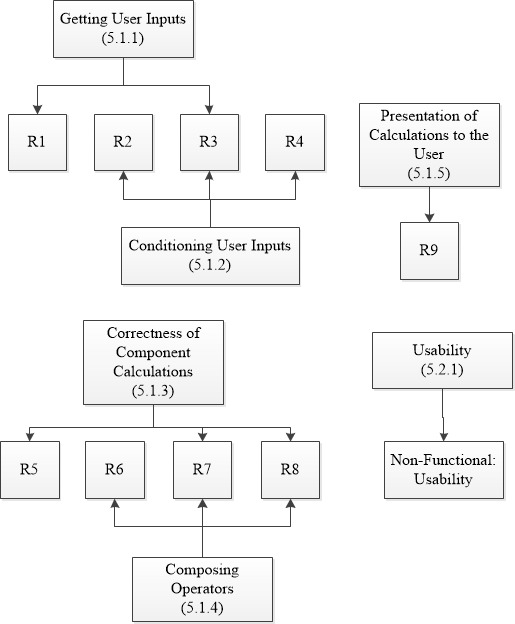
\includegraphics[width=0.66\textwidth]{figures/ReqToTest.png}
		}
		\caption{\label{Fig:req2tests} Traceability Graph Showing the 
		Connections Requirements and Test Suites}
	\end{center}
\end{figure}
				
\newpage				
				
\section{Unit Testing}
		
As shown by the system test description (Section \ref{testplan_highlevel}), the 
system and integration testing of the \prognameAbbrv{} tool can be divided into 
several unique steps. However, these tests do not cover all possible code paths 
such that 100\% code coverage can be achieved. The unit tests were created in 
addition to the functional requirements tests to realize this goal. Unit 
testing is divided by modules.

\subsection{Control Flow Unit Tests}
These tests are designed to exercise all code paths in the 
\texttt{ControlFlow.cs} file in the \texttt{CompanionCubeCalculator.csproj} 
project file. They are implemented in the \texttt{ControlTests.cs} file in the 
\texttt{UnitTests\_CompanionCubeCalculator.csproj} project file. These projects 
are collected in the \texttt{CompanionCubeCalculator.sln} solution file.

\begin{enumerate}
	
	\item{unittest-controlinit}
	
	Type: Functional, Automatic, Unit
	
	Initial State: New Session
	
	Input: $ControlFlow.Initialize()$
	
	Output: $TRUE$
	
	User Message: Parser initialized.
	
	How test will be performed: Unit Testing\\
	
	\item{unittest-controlcondition}
	
	Type: Functional, Automatic, Unit
	
	Initial State: New Session
	
	Input: \texttt{"x + y"}, $TRUE$
	
	Output: \texttt{"x+y"}
	
	User Message: -
	
	How test will be performed: Unit Testing\\
	
	\item{unittest-controlgetfiletypes}
	
	Type: Functional, Automatic, Unit
	
	Initial State: New Session
	
	Input: $ControlFlow.GetValidFileTypes()$
	
	Output: \texttt{"*.txt"}
	
	User Message: -
	
	How test will be performed: Unit Testing\\
	
	\item{unittest-controlextractvars}
	
	Type: Functional, Automatic, Unit
	
	Initial State: New Session
	
	Input: \texttt{ "x+y" }
	
	Output: \texttt{ \{ "x", "y" \}}
	
	User Message: -
	
	How test will be performed: Unit Testing\\
	
	\item{unittest-controlgetvarinfo}
	
	Type: Functional, Automatic, Unit
	
	Initial State: New Session
	
	Input: \texttt{ \{ "x+y", "x,2,4\textbackslash ny,3,5" \} }
	
	Output: \texttt{ \{ \{ "x", "2", "4" \}, \{ "y", "3", "5" \} \}}
	
	User Message: -
	
	How test will be performed: Unit Testing\\
	
	\item{unittest-controlfile}
	
	Type: Functional, Automatic, Unit
	
	Initial State: New Session
	
	Input: \texttt{@"TestFiles/test.txt"}
	
	Output: \texttt{ \{ "x+y", "x,2,4\textbackslash ny,3,5" \} }
	
	User Message: -
	
	How test will be performed: Unit Testing\\
	
\end{enumerate}

\subsection{User Input Unit Tests}
\label{unit_inputs}
These tests are designed to exercise all code paths in the \texttt{Input.cs} 
file in the \texttt{CompanionCubeCalculator.csproj} project file. They are 
implemented in the \texttt{InputTests.cs} file in the 
\texttt{UnitTests\_CompanionCubeCalculator.csproj} project file. These projects 
are collected in the \texttt{CompanionCubeCalculator.sln} solution file.

\paragraph{File I/O}
\begin{enumerate}
	
	\item{unittest-fileinput}
	
	Type: Functional, Automatic, Unit
	
	Initial State: New Session
	
	Input: File containing:
	\begin{lstlisting}
	x + y
	x,2,4
	y,3,5
	\end{lstlisting}
	
	Output: \{ "x+y", "x,2,4\textbackslash ny,3,5" \}
	
	User Message: - 
	
	How test will be performed: Unit Test\\
	
	\item{unittest-fileinputwithequals}
	
	Type: Functional, Automatic, Unit
	
	Initial State: New Session
	
	Input: File containing:
	\begin{lstlisting}
	f(V) = x + y
	x,2,4
	y,3,5
	\end{lstlisting}
	
	Output: \{ "x+y", "x,2,4\textbackslash ny,3,5" \}
	
	User Message: - 
	
	How test will be performed: Unit Test\\
	
	\item{unittest-emptyfile}
	
	Type: Functional, Automatic, Unit
	
	Initial State: New Session
	
	Input: File containing no information
	
	Output: $NULL$
	
	User Message: Error: The file is empty.
	
	How test will be performed: Unit Test\\
	
	\item{unittest-invalidfiletype}
	
	Type: Functional, Automatic, Unit
	
	Initial State: New Session
	
	Input: File with an unsupported extension
	
	Output: $NULL$
	
	User Message: Error: Cannot read files of this type.
	
	How test will be performed: Unit Test\\
	
	\item{unittest-input\_noFunctionFile}
	
	Type: Functional, Automatic, Unit
	
	Initial State: New Session
	
	Input: A file containing:
	\begin{lstlisting}
	x,2,4
	y,3,5
	\end{lstlisting}
	
	Output: $NULL$
	
	User Message: Error: The first line of the file is not an equation or the 
	equation contains ','.
	
	How test will be performed: Unit Test\\
	
	\item{unittest-noFile}
	
	Type: Functional, Automatic, Unit
	
	Initial State: New Session
	
	Input: A file that does not exist
	
	Output: $NULL$
	
	User Message: Error: The specified file does not exist.
	
	How test will be performed: Unit Test\\
	
	\item{unittest-badFileInput}
	
	Type: Functional, Automatic, Unit
	
	Initial State: New Session
	
	Input: File that cannot be read
	
	Output: $NULL$
	
	User Message: Error: Cannot read files of this type.
	
	How test will be performed: Unit Test\\
\end{enumerate}

\paragraph{Getters}
\begin{enumerate}
	\item{unittest-testgetlinedelimiter}
	
	Type: Functional, Automatic, Unit
	
	Initial State: New Session
	
	Input: -
	
	Output: \texttt{"\textbackslash r\textbackslash n"}
	
	User Message: - 
	
	How test will be performed: Unit Testing\\
	
	\item{unittest-testgetfielddelimiter}
	
	Type: Functional, Automatic, Unit
	
	Initial State: New Session
	
	Input: -
	
	Output: \texttt{","}
	
	User Message: - 
	
	How test will be performed: Unit Testing\\
	
	\item{unittest-testgetfiletypes}
	
	Type: Functional, Automatic, Unit
	
	Initial State: New Session
	
	Input: -
	
	Output: \texttt{"*.txt"}
	
	User Message: - 
	
	How test will be performed: Unit Testing\\
	
\end{enumerate}

\subsection{Interval Data Structure and Interval Conversion Unit Tests}
These tests are designed to exercise all code paths in the 
\texttt{IntervalStruct.cs} and \texttt{IntervalConversion.cs}
files in the \texttt{CompanionCubeCalculator.csproj} project file. They are 
implemented in the \texttt{IntervalTests.cs} file in the \\
\texttt{UnitTests\_CompanionCubeCalculator.csproj} project file. These projects 
are collected in the \texttt{CompanionCubeCalculator.sln} solution file.

\paragraph{Interval Data Structure}
\begin{enumerate}
	
	\item{unittest-intervaldatastructuresetters}
	
	Type: Functional, Automatic, Unit
	
	Initial State: New Session
	
	Input: \texttt{ "x", "3", "4"}, $False$, $False$
	
	Changes: $min = 2$, $max = 5$, $leftBoundClosed = TRUE$, $rightBoundClosed 
	= TRUE$
	
	Output: \texttt{ "x"}, $2$, $5$, $True$, $True$
	
	User Message: - 
	
	How test will be performed: Unit Testing\\
	
	\item{unittest-intervaldatastructuresetvarname}
	
	Type: Functional, Automatic, Unit
	
	Initial State: New Session
	
	Input: \texttt{ "x", "3", "4"}, $False$, $False$
	
	Changes: $varName = y$
	
	Output: \texttt{ "y"}, $3$, $4$, $False$, $False$
	
	User Message: -
	
	How test will be performed: Unit Testing\\
	
\end{enumerate}

\paragraph{Interval Conversion}
\begin{enumerate}
	
	\item{unittest-intervalconversionmissingbounds}
	
	Type: Functional, Automatic, Unit
	
	Initial State: New Session
	
	Input: \texttt{"x"}
	
	Output: \{\}
	
	User Message: Error: No fields found for variable (Line n). Skipping line.
	
	How test will be performed: Unit Testing\\
	
	\item{unittest-intervalconversionemptybounds}
	
	Type: Functional, Automatic, Unit
	
	Initial State: New Session
	
	Input: \texttt{"x,,"}
	
	Output: \{   \}
	
	User Message: Error: No values provided for either interval bound.
	
	How test will be performed: Unit Testing\\
	
	\item{unittest-intervalconversionmissingvarname}
	
	Type: Functional, Automatic, Unit
	
	Initial State: New Session
	
	Input: \texttt{"3.0,4.0"}
	
	Output: \{   \}
	
	User Message: Error: Intervals must have an associated variable name.
	
	How test will be performed: Unit Testing\\
	
	\item{unittest-intervalconversionemptyvarname}
	
	Type: Functional, Automatic, Unit
	
	Initial State: New Session
	
	Input: \texttt{",3.0,4.0"}
	
	Output: \{   \}
	
	User Message: Error: Intervals must have an associated variable name.
	
	How test will be performed: Unit Testing\\
	
	\item{unittest-intervalconversiontoomanyfields}
	
	Type: Functional, Automatic, Unit
	
	Initial State: New Session
	
	Input: \texttt{"x,3,4,5"}
	
	Output: \{   \}
	
	User Message: Error: Encountered a variable with more than three fields 
	(Line n). Skipping line.
	
	How test will be performed: Unit Testing\\
	
\end{enumerate}

\subsection{Equation Data Structure and Equation Conversion Unit Tests}
These tests are designed to exercise all code paths in the 
\texttt{EquationStruct.cs} and \texttt{EquationConversion.cs} 
files in the \texttt{CompanionCubeCalculator.csproj} project file. They are 
implemented in the \texttt{EquationTests.cs} file in the \\
\texttt{UnitTests\_CompanionCubeCalculator.csproj} project file. These projects 
are collected in the \texttt{CompanionCubeCalculator.sln} solution file.

\paragraph{Equation Data Structure}

\subparagraph{Constructors}
\begin{enumerate}
	
	\item{unittest-equationdatastructurenoop}
	
	Type: Functional, Automatic, Unit
	
	Initial State: New Session
	
	Input: \texttt{"", ""}, $NULL$, $NULL$
	
	Output: \texttt{Exception}
	
	User Message: Error: Equation structures must be assigned an operator 
	during initialization.
	
	How test will be performed: Unit Testing\\
	
	\item{unittest-equationdatastructureconstructnulls}
	
	Type: Functional, Automatic, Unit
	
	Initial State: New Session
	
	Input: \texttt{"+", "x"}, $NULL$, $NULL$
	
	Output: \Tree[.$+:x$ [.$null$  ] [.$null$  ] ]
	
	User Message: -
	
	How test will be performed: Unit Testing\\
	
	\item{unittest-equationdatastructureconstruct}
	
	Type: Functional, Automatic, Unit
	
	Initial State: New Session
	
	Input: \texttt{"+", "x"}, \Tree[.$VAR:y$ [.$null$  ] [.$null$  ] ], 
	\Tree[.$VAR:z$ 	[.$null$  ] [.$null$  ] ]
	
	Output: \Tree[.$+:x$ [.$VAR:y$ [.$null$  ] [.$null$  ] ]  [.$VAR:z$  
	[.$null$  ] [.$null$  ]  ] ] 
	
	User Message: -
	
	How test will be performed: Unit Testing\\
	
\end{enumerate}

\subparagraph{Getters}
\begin{enumerate}
	
	\item{unittest-equationdatastructuresetvarname}
	
	Type: Functional, Automatic, Unit
	
	Initial State: New Session
	
	Input: \Tree[.$+:x$ [.$null$  ] [.$null$  ] ], \texttt{y}
	
	Output: \Tree[.$+:y$ [.$null$  ] [.$null$  ] ]
	
	User Message: -
	
	How test will be performed: Unit Testing\\
	
	\item{unittest-equationdatastructuresetleftop}
	
	Type: Functional, Automatic, Unit
	
	Initial State: New Session
	
	Input: \Tree[.$+:x$ [.$null$  ] [.$null$  ] ], \Tree[.$VAR:y$ [.$null$  ] 
	[.$null$  ] ]
	
	Output: \Tree[.$+:x$ [.$VAR:y$ [.$null$  ] [.$null$  ] ]  [.$null$  ] ] 
	
	User Message: -
	
	How test will be performed: Unit Testing\\
	
	\item{unittest-equationdatastructuresetrightop}
	
	Type: Functional, Automatic, Unit
	
	Initial State: New Session
	
	Input: \Tree[.$+:x$ [.$null$  ] [.$null$  ] ], \Tree[.$VAR:z$ [.$null$  ] 
	[.$null$  ] ]
	
	Output: \Tree[.$+:x$  [.$null$  ] [.$VAR:z$ [.$null$  ] [.$null$  ] ] ] 
	
	User Message: -
	
	How test will be performed: Unit Testing\\
	
\end{enumerate}

\paragraph{Equation Conversion}
\begin{enumerate}
	
	\item{unittest-equationconversionconfignoops}
	
	Type: Functional, Automatic, Unit
	
	Initial State: New Session
	
	Input: $new OperatorStruct[] \{ \}$, $Solver.GetValidTerminators()$
	
	Output: $FALSE$
	
	User Message: Error: No operators were passed to the parser.
	
	How test will be performed: Unit Testing\\
	
	\item{unittest-equationconversionconfigunary}
	
	Type: Functional, Automatic, Unit
	
	Initial State: New Session
	
	Input: $new OperatorStruct[] \{ new OperatorStruct("-", 5, true, 
	false, false, false) \} $, $Solver.GetValidTerminators()$
	
	Output: $TRUE$
	
	User Message: -
	
	How test will be performed: Unit Testing\\
	
	\item{unittest-equationconversionconfigbinary}
	
	Type: Functional, Automatic, Unit
	
	Initial State: New Session
	
	Input: $new OperatorStruct[] \{ new OperatorStruct("-", 5, false, 
			true, false, false) \}$, $Solver.GetValidTerminators()$
	
	Output: $TRUE$
	
	User Message: -
	
	How test will be performed: Unit Testing\\
	
	\item{unittest-equationconversionconfigternary}
	
	Type: Functional, Automatic, Unit
	
	Initial State: New Session
	
	Input: $new OperatorStruct[] \{ new OperatorStruct("\&", 5, false, 
			false, true, false) \}$, $Solver.GetValidTerminators()$
	
	Output: $FALSE$
	
	User Message: Error: The parser cannot process the \& operator.
	
	How test will be performed: Unit Testing\\
	
	\item{unittest-equationconversionconfigunbalancedleftterm}
	
	Type: Functional, Automatic, Unit
	
	Initial State: New Session
	
	Input: $Solver.GetValidOperators()$, $new string[] \{ "(", "" \}$
	
	Output: $FALSE$
	
	User Message: Error: An unbalanced left terminator token was encountered 
	(().
	
	How test will be performed: Unit Testing\\
	
	\item{unittest-equationconversionconfigunbalancedrightterm}
	
	Type: Functional, Automatic, Unit
	
	Initial State: New Session
	
	Input: $Solver.GetValidOperators()$, $new string[] \{ "", ")" \}$
	
	Output: $FALSE$
	
	User Message: Error: An unbalanced right terminator token was encountered 
	()).
	
	How test will be performed: Unit Testing\\
	
	\item{unittest-equationconversionparseunary}
	
	Type: Functional, Automatic, Unit
	
	Initial State: New Session
	
	Input: \texttt{"-x"}, $new OperatorStruct("-", 5, true, false, false, 
	false)$
	
	Output: \Tree[.$-:$ [.$VAR:x$ [.$null$  ] [.$null$  ] ] [.$null$  ]  ] 
	
	User Message: -
	
	How test will be performed: Unit Testing\\
	
	\item{unittest-equationconversion\_missingFunctionValue1}
	
	Type: Functional, Automatic, Unit
	
	Initial State: New Session
	
	Input: \texttt{"x+"}
	
	Output: $NULL$
	
	User Message: Error: Could not find the end of the equation. 
	
	How test will be performed: Unit Test\\
	
	\item{unittest-equationconversion\_missingFunctionValue2}
	
	Type: Functional, Automatic, Unit
	
	Initial State: New Session
	
	Input: \texttt{"*x"}
	
	Output:	$NULL$
	
	User Message: Error: Unrecognized sequence encountered during Atomic 
	Equation parsing. Remaining equation = *x.
	
	How test will be performed: Unit Test\\
	
	\item{unittest-equationconversion\_missingFunctionValue3}
	
	Type: Functional, Automatic, Unit
	
	Initial State: New Session
	
	Input: \texttt{"x+*y"}
	
	Output:	$NULL$
	
	User Message: Error: Unrecognized sequence encountered during Atomic 
	Equation parsing. Remaining equation = *y.
	
	How test will be performed: Unit Test\\
	
\end{enumerate}

\subsection{Variable Consolidation Unit Tests}
These tests are designed to exercise all code paths in the 
\texttt{Consolidate.cs} 
file in the \texttt{CompanionCubeCalculator.csproj} project file. They are 
implemented in the \texttt{VariableConsolidationTests.cs} file in the \\
\texttt{UnitTests\_CompanionCubeCalculator.csproj} project file. These projects 
are collected in the \texttt{CompanionCubeCalculator.sln} solution file.

\begin{enumerate}
	
	\item{unittest-consolidatetestinit}
	
	Type: Functional, Automatic, Integration
	
	Initial State: New Session
	
	Input: -
	
	Output: $TRUE$
	
	User Message: -
	
	How test will be performed: Unit Testing\\
	
	\item{unittest-consolidatetestinit}
	
	Type: Functional, Automatic, Integration
	
	Initial State: New Session
	
	Input: -
	
	Output: $TRUE$
	
	User Message: -
	
	How test will be performed: Unit Testing\\
	
	\item{unittest-consolidatenoops}
	
	Type: Functional, Automatic, Integration
	
	Initial State: New Session
	
	Input: $ConvertAndCheckInputs(\texttt{"x+y"}, \texttt{"x,2,3 \textbackslash 
		ny,4,5"}, \{ \},\\ Solver.GetValidTerminators())$
	
	Output: $successCode = -1$
	
	User Message: Error: No operators were passed to the parser.
	
	How test will be performed: Unit Testing\\
	
	\item{unittest-consolidatenorightterm}
	
	Type: Functional, Automatic, Integration
	
	Initial State: New Session
	
	Input: $ConvertAndCheckInputs(\texttt{"x+y"}, \texttt{"x,2,3 \textbackslash 
		ny,4,5"},\\ Solver.GetValidOperators(), \{ \{ ``(" \} \})$
	
	Output: $successCode = -1$
	
	User Message: Error: An unbalanced left terminator token was encountered 
	(``(")
	
	How test will be performed: Unit Testing\\
	
	\item{unittest-consolidatenoleftterm}
	
	Type: Functional, Automatic, Integration
	
	Initial State: New Session
	
	Input: $ConvertAndCheckInputs(\texttt{"x+y"}, \texttt{"x,2,3 \textbackslash 
		ny,4,5"},\\ Solver.GetValidOperators(), \{ \{ ``)" \} \})$
	
	Output: $successCode = -1$
	
	User Message: Error: An unbalanced right terminator token was encountered 
	(``)")
	
	How test will be performed: Unit Testing\\
	
	\item{unittest-consolidatesimpleinputs}
	
	Type: Functional, Automatic, Integration
	
	Initial State: New Session
	
	Input: $ConvertAndCheckInputs(\texttt{"x+y"}, \texttt{"x,2,3 \textbackslash 
		ny,4,5"}, Solver.GetValidOperators(),\\ Solver.GetValidTerminators())$
	
	Output: \Tree[.$+$ [.$x$  ] [.$y$  ] ], \{ $x = [2,3]$, $y = [4,5]$ \}
	
	User Message: - 
	
	How test will be performed: Unit Testing\\
	
	\item{unittest-consolidateextractvariables}
	
	Type: Functional, Automatic, Integration
	
	Initial State: New Session
	
	Input: $ConvertAndCheckInputs(\texttt{"x+y"}, \texttt{"x,2,3 \textbackslash 
		ny,4,5"}, Solver.GetValidOperators(),\\ 
		Solver.GetValidTerminators());\\ Consolidate.GetIntervalStructList()$
	
	Output: \{ $x = [2,3]$, $y = [4,5]$ \}
	
	User Message: - 
	
	How test will be performed: Unit Testing\\
	
	\item{unittest-consolidateincompleteequation}
	
	Type: Functional, Automatic, Integration
	
	Initial State: New Session
	
	Input: \texttt{"", "x,2,3\textbackslash n"}
	
	Output: $successCode = -1$
	
	User Message: Error: Unrecognized sequence encountered during Atomic 
	Equation parsing. Remaining equation = 
	
	How test will be performed: Unit Testing\\
	
	
\end{enumerate}

\subsection{Operator Data Structure and Range Solver Unit Tests}
These tests are designed to exercise all code paths in the 
\texttt{OperatorStruct.cs} and \texttt{Solver.cs} 
files in the \texttt{CompanionCubeCalculator.csproj} project file. They are 
implemented in the \texttt{SolverTests.cs} file in the \\
\texttt{UnitTests\_CompanionCubeCalculator.csproj} project file. These projects 
are collected in the \texttt{CompanionCubeCalculator.sln} solution file.

\paragraph{Operator Data Structure}
\begin{enumerate}
	
	\item{unittest-operatordatastructureconstructor}
	
	Type: Functional, Automatic, Unit
	
	Initial State: New Session
	
	Input: \texttt{"+"}, $1, false, true, false, true$
	
	Output: $OperatorStruct(\texttt{"+"},1,false,true,false,true)$
	
	User Message: - 
	
	How test will be performed: Unit Testing\\
	
	\item{unittest-operatordatastructuremissingsym}
	
	Type: Functional, Automatic, Unit
	
	Initial State: New Session
	
	Input: \texttt{""}, $1, false, true, false, true$
	
	Output: \texttt{Exception}
	
	User Message: Error: Cannot have an operator with no representative symbol.
	
	How test will be performed: Unit Testing\\
	
	\item{unittest-operatordatastructurelowprecedence}
	
	Type: Functional, Automatic, Unit
	
	Initial State: New Session
	
	Input: \texttt{"+"}, $0, false, true, false, true$
	
	Output: \texttt{Exception}
	
	User Message: Error: Precedence values must be greater than 0.
	
	How test will be performed: Unit Testing\\
	
	\item{unittest-operatordatastructureoverloadedtype1}
	
	Type: Functional, Automatic, Unit
	
	Initial State: New Session
	
	Input: \texttt{"+"}, $1, true, true, false, true$
	
	Output: \texttt{Exception}
	
	User Message: Error: An operator cannot be overloaded to be unary, binary, 
	and ternary.
	
	How test will be performed: Unit Testing\\
	
	\item{unittest-operatordatastructureoverloadedtype2}
	
	Type: Functional, Automatic, Unit
	
	Initial State: New Session
	
	Input: \texttt{"+"}, $1, false, true, true, true$
	
	Output: \texttt{Exception}
	
	User Message: Error: An operator cannot be overloaded to be unary, binary, 
	and ternary.
	
	How test will be performed: Unit Testing\\
	
	\item{unittest-operatordatastructureoverloadedtype3}
	
	Type: Functional, Automatic, Unit
	
	Initial State: New Session
	
	Input: \texttt{"+"}, $1, true, false, true, true$
	
	Output: \texttt{Exception}
	
	User Message: Error: An operator cannot be overloaded to be unary, binary, 
	and ternary.
	
	How test will be performed: Unit Testing\\
	
	\item{unittest-operatordatastructurenotype}
	
	Type: Functional, Automatic, Unit
	
	Initial State: New Session
	
	Input: \texttt{"+"}, $1, false, false, false, true$
	
	Output: \texttt{Exception}
	
	User Message: Error: Operators must be assigned a number of operands type.
	
	How test will be performed: Unit Testing\\
	
\end{enumerate}

\paragraph{Range Solver}
\begin{enumerate}
	
	\item{unittest-solvernoequation}
	
	Type: Functional, Automatic, Integration
	
	Initial State: New Session
	
	Input: $null, x = [1,2]$
	
	Output: \texttt{Exception}
	
	User Message: Error: No information was provided for the equation.
	
	How test will be performed: Unit Testing\\
	
	\item{unittest-solverunknownop}
	
	Type: Functional, Automatic, Integration
	
	Initial State: New Session
	
	Input: \Tree[.$**:$ [.$VAR:x$ [.$null$  ] [.$null$  ] ]  [.$VAR:x$  
	[.$null$  ] [.$null$  ]  ] ], $x = [2,3]$
	
	Output: $NULL$
	
	User Message: Error: An unsupported operation was encountered while solving 
	for the range of the equation (Unknown operator).
	
	How test will be performed: Unit Testing\\
	
	\item{unittest-solvermissingintervals}
	
	Type: Functional, Automatic, Integration
	
	Initial State: New Session
	
	Input: \Tree[.$VAR:x$  [.$null$  ] [.$null$  ]  ], $\{ \}$
	
	Output: $NULL$
	
	User Message: Error: Could not find an associated interval for variable x.
	
	How test will be performed: Unit Testing\\
	
	\item{unittest-solverconstantfunction}
	
	Type: Functional, Automatic, Integration
	
	Initial State: New Session
	
	Input: \Tree[.$CONST:42$  [.$null$  ] [.$null$  ]  ], $\{ \}$
	
	Output: $[42,42]$
	
	User Message: -
	
	How test will be performed: Unit Testing\\
	
	\item{unittest-solvervariablefunction}
	
	Type: Functional, Automatic, Integration
	
	Initial State: New Session
	
	Input: \Tree[.$VAR:x$  [.$null$  ] [.$null$  ]  ], $\{ x = [2,3] \}$
	
	Output: $[2,3]$
	
	User Message: -
	
	How test will be performed: Unit Testing\\
	
	\item{unittest-solveradditionleftsidenull}
	
	Type: Functional, Automatic, Integration
	
	Initial State: New Session
	
	Input: \Tree[.$+:$  [.$():$ [.$/:$  [.$VAR:y$  [.$null$  ] [.$null$  ]  ] 
	[.$VAR:z$  [.$null$  ] [.$null$  ]  ]  ]  ] [.$VAR:x$  [.$null$  ] 
	[.$null$  ]  ]  ], \\$\{ x = [2,4], y = [-3,5], z = [-1,1] \}$
	
	Output: $NULL$
	
	User Message: Error: An unsupported operation was encountered while solving 
	for the range of the equation (Mixed interval division).
	
	How test will be performed: Unit Testing\\
	
	\item{unittest-solversubtractionleftsidenull}
	
	Type: Functional, Automatic, Integration
	
	Initial State: New Session
	
	Input: \Tree[.$-:$  [.$():$ [.$/:$  [.$VAR:y$  [.$null$  ] [.$null$  ]  ] 
	[.$VAR:z$  [.$null$  ] [.$null$  ]  ]  ]  ] [.$VAR:x$  [.$null$  ] 
	[.$null$  ]  ]  ], \\$\{ x = [2,4], y = [-3,5], z = [-1,1] \}$
	
	Output: $NULL$
	
	User Message: Error: An unsupported operation was encountered while solving 
	for the range of the equation (Mixed interval division).
	
	How test will be performed: Unit Testing\\
	
	\item{unittest-solvermultiplicationleftsidenull}
	
	Type: Functional, Automatic, Integration
	
	Initial State: New Session
	
	Input: \Tree[.$*:$  [.$():$ [.$/:$  [.$VAR:y$  [.$null$  ] [.$null$  ]  ] 
	[.$VAR:z$  [.$null$  ] [.$null$  ]  ]  ]  ] [.$VAR:x$  [.$null$  ] 
	[.$null$  ]  ]  ], \\$\{ x = [2,4], y = [-3,5], z = [-1,1] \}$
	
	Output: $NULL$
	
	User Message: Error: An unsupported operation was encountered while solving 
	for the range of the equation (Mixed interval division).
	
	How test will be performed: Unit Testing\\
	
	\item{unittest-solverdivisionleftsidenull}
	
	Type: Functional, Automatic, Integration
	
	Initial State: New Session
	
	Input: \Tree[.$/:$  [.$():$ [.$/:$  [.$VAR:y$  [.$null$  ] [.$null$  ]  ] 
	[.$VAR:z$  [.$null$  ] [.$null$  ]  ]  ]  ] [.$VAR:x$  [.$null$  ] 
	[.$null$  ]  ]  ], \\$\{ x = [2,4], y = [-3,5], z = [-1,1] \}$
	
	Output: $NULL$
	
	User Message: Error: An unsupported operation was encountered while solving 
	for the range of the equation (Mixed interval division).
	
	How test will be performed: Unit Testing\\
	
	\item{unittest-solverexponentleftsidenull}
	
	Type: Functional, Automatic, Integration
	
	Initial State: New Session
	
	Input: \Tree[.$\wedge:$  [.$():$ [.$/:$  [.$VAR:y$  [.$null$  ] [.$null$  
	]  ]  [.$VAR:z$  [.$null$  ] [.$null$  ]  ]  ]  ] [.$CONST:4$  [.$null$  ] 
	[.$null$  ]  ]  ], \\$\{ y = [-3,5], z = [-1,1] \}$
	
	Output: $NULL$
	
	User Message: Error: An unsupported operation was encountered while solving 
	for the range of the equation (Mixed interval division).
	
	How test will be performed: Unit Testing\\

\end{enumerate}

\subsection{Output Unit Tests}
These tests are designed to exercise all code paths in the \texttt{Output.cs} 
file in the \texttt{CompanionCubeCalculator.csproj} project file. They are 
implemented in the \texttt{OutputTests.cs} file in the 
\texttt{UnitTests\_CompanionCubeCalculator.csproj} project file. These projects 
are collected in the \texttt{CompanionCubeCalculator.sln} solution file.

\begin{enumerate}
	
	\item{unittest-outputopenstructure}
	
	Type: Functional, Automatic, Integration
	
	Initial State: New Session
	
	Input: $x = (2,4), true$
	
	Output: \texttt{x = (2, 4)}
	
	User Message: - 
	
	How test will be performed: Unit Testing\\
	
	\item{unittest-outputclosedleftstructure}
	
	Type: Functional, Automatic, Integration
	
	Initial State: New Session
	
	Input: $x = [2,4), true$
	
	Output: \texttt{x = [2, 4)}
	
	User Message: - 
	
	How test will be performed: Unit Testing\\
	
	\item{unittest-outputclosedrightstructure}
	
	Type: Functional, Automatic, Integration
	
	Initial State: New Session
	
	Input: $x = (2,4], true$
	
	Output: \texttt{x = (2, 4]}
	
	User Message: - 
	
	How test will be performed: Unit Testing\\
	
	\item{unittest-outputconstwithname}
	
	Type: Functional, Automatic, Integration
	
	Initial State: New Session
	
	Input: $CONST: 3, true$
	
	Output: \texttt{CONST: 3}
	
	User Message: - 
	
	How test will be performed: Unit Testing\\
	
	\item{unittest-outputconstnoname}
	
	Type: Functional, Automatic, Integration
	
	Initial State: New Session
	
	Input: $CONST: 3, false$
	
	Output: \texttt{CONST: 3}
	
	User Message: - 
	
	How test will be performed: Unit Testing\\
	
	\item{unittest-outputlongresult}
	
	Type: Functional, Automatic, Integration
	
	Initial State: New Session
	
	Input: $x = [0.333333333333, 0.66666666666666], false$
	
	Output: \texttt{[0.333333333333, \textbackslash n 0.66666666666666]}
	
	User Message: - 
	
	How test will be performed: Unit Testing\\
	
\end{enumerate}

%\bibliographystyle{plainnat}

%\bibliography{SRS}

\newpage

\section{Appendix: Usability Testing}
\label{appendix_userstudy}
An informal user study was conducted as part of the \progname{} test suite, 
where participants were recruited from the examiner's lab. Participants were 
sent a compressed file containing the program, user manual, and instructions 
and asked to complete it on their own time. The instructions file contained a 
URL to the associated study questionnaire. 

The instructions that were sent to participants can be found at: 

\begin{center}
	\href{https://github.com/GenevaS/CAS741/tree/master/Doc/TestReport/UserStudy}{https://github.com/GenevaS/CAS741/tree/master/Doc/TestReport/UserStudy}
\end{center}

\subsection{Tasks}
User study participants were asked to complete two tasks given the information: 

$$\frac{2(x + y)^2}{3^z}$$

where

$$x = [1, 2], y = [3, 4], z = [5, 6]$$

The first task was to input the information directly into the GUI and the 
second task was to load the information into the program via a file.

Participants were free to access the program user guide as they saw fit. 

\subsection{Questionnaire}
This survey were designed to accompany the user study. The questionnaire was 
distributed as a Google Form. All Likert scale questions were from 1 to 5, 
where 1 is ``Strongly Disagree" and 5 is ``Strongly Agree".

\subsubsection{Test Results (Round values as necessary)}
\begin{enumerate}
	\item (Long Answer) What range value did you calculate in Task 1?
	\item (Long Answer) What was the resulting equation tree from Task 1?
	\item (Long Answer) What range value did you calculate in Task 2?
	\item (Long Answer) What was the resulting equation tree from Task 2?
\end{enumerate}

\subsubsection{Software Usability}
\paragraph{Task 1: Entering values directly into the GUI}
\begin{enumerate}
	\item (Likert Scale)I found it easy to find the input mechanism for 
	entering 
	the equation into the GUI.
	
	\item (Likert Scale) I found it easy to use the function input mechanism.
	
	\item (Likert Scale) I found it easy to find the input mechanism for 
	entering variable domains into the GUI. 
	
	\item (Likert Scale) I found it easy to use the variable domain input 
	mechanism. 
\end{enumerate}

\paragraph{Task 2: Loading values into the program from a file}
\begin{enumerate}
	\item (Likert Scale) I found it easy to find the option to load from a file.
\end{enumerate}

\paragraph{Understanding the Results}
\begin{enumerate}
	\item (Likert Scale) I found it easy to find the calculated range in the 
	GUI.
	
	\item (Likert Scale) I found it easy to understand the calculated range. 
	
	\item (Likert Scale) I found it easy to understand the sequence of steps 
	required to use the software. 
	
	\item (Long answer) Describe any interactions with the program that 
	confused you during the tasks.
	
	\item (Long answer)  Do you have any suggestions for improving the process 
	flow of the tool?
\end{enumerate}


\end{document}